\documentclass[../memory.tex]{subfiles}

\begin{document}
\chapter{Planning}
\section{Task division}
Recurrent Travel is supported by a team of four professionals responsible for
the application development. One has expertise in frontend, one in full stack
development, and the remaining two have expertise in backend development and
devops. Despite each member having specific expertise in their respective
fields, the team is cross-functional, and the project development can be carried
out by them without the need for external dependencies.
\\
The project consists of the following elements:
\begin{enumerate}[label = -]
	\item A user interface application to allow the user to interact with the
	      application.
	\item Four services that include the backend server logic, database management
	      and data scrapping.
	\item A backend communication system, such as a queue, to allow the different
	      services to communicate between them.
\end{enumerate}
Taking into account this proposal and the abilities of each team member of the
team, the division of the responsibilities is distributed considering that the
majority of the work focuses on backend development. Therefore, most part of the
resources are assigned to the backend, with specialised members leading and
executing tasks related to such area. The member with strong knowledge in
interface design and frontend development will be assigned to the development of
the user interface, user experience and frontend business logic. The planning
and overall structure of the project are taken care by the member with knowledge
in software architecture and design. Code quality, testing and similar aspects
are elements that each member will have to handle by themselves. Lastly, the
entire development is overseen and coordinated by a project leader.
\\[8pt]
With the previous parameters in mind, the initial planning consisted in the
creation of the tickets in order to be able to accomplish the expected tasks,
which were defined every two weeks. It is also worth mentioning that tasks could
vary in time, as it is really hard to detect possible problems or issues in the
development, when planning the tasks.
\begin{figure}[H]
	\centering
	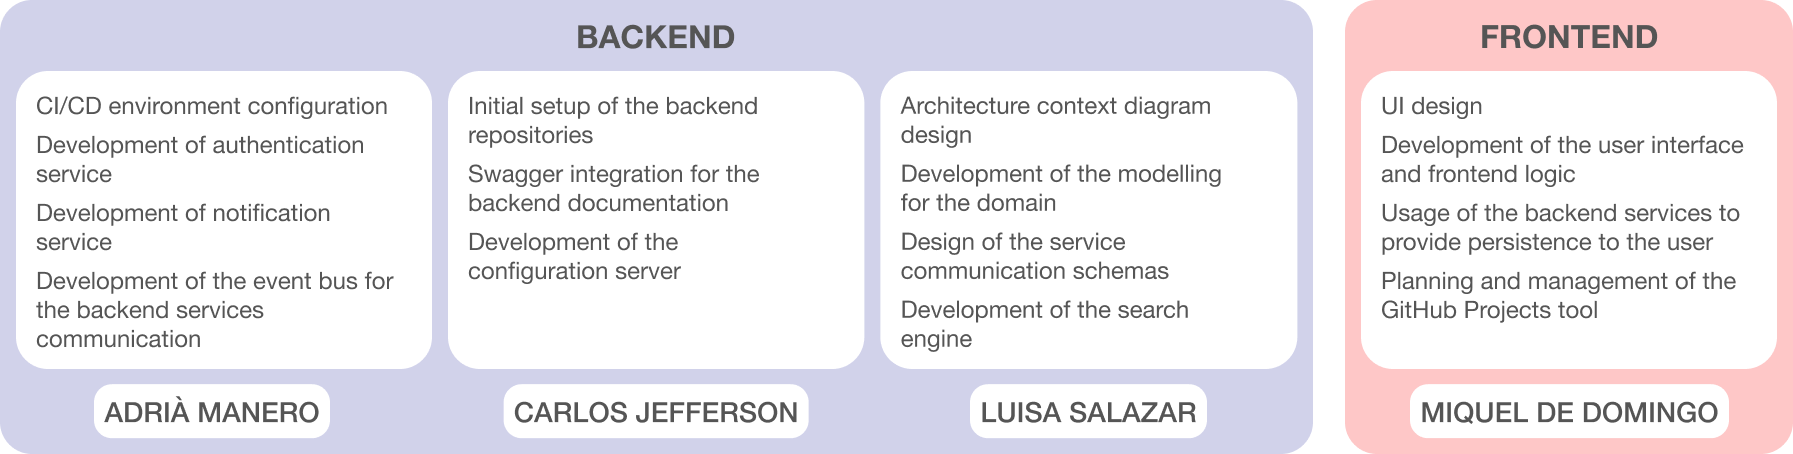
\includegraphics[width=\textwidth]{./assets/planning-organization.png}
	\caption{Task distribution as a schema}
\end{figure}
It is important to point out that during the development of the process the each
member of the team is not exclusively focused in the tasks described above,
rather it contributes and collaborates to the execution of the assigned tickets
to other members, when help is needed, helping diminish the handicaps of the
project.
\\
At the same time, there are tasks that are executed by all members of the team
and are part of the global work required to develop the project:
\begin{enumerate}[label = -]
	\item Definition of the rules in terms of code (using tools that validate a
	      certain style of code, also known as linters) and to contribute to each
	      repository.
	\item Planning of the expected work to be finished for each sprint.
	\item Code review of each developed task, in order to provide a second opinion
	      in the code \emph{to be merged}.
	\item Study, evaluation and proposal of technologies both for development and
	      deployment of the systems to be developed.
\end{enumerate}
Being more specific, the following are the tasks for each team member.
\begin{enumerate}[label =]
	\item\textbf{Miquel de Domingo - Frontend}
	\begin{enumerate}[label = -]
		\item\textbf{Website design}. Involves all the proposed user interface
		designs that the application will have, including responsive designs
		for small screen devices, since the application will be accessed
		through the browser.
		\item\textbf{Configuration of CI and CD}. This task involves design and
		execution of strategies that provide frontend repository with
		continuous integration and deployment strategies.
		\item\textbf{Interactivity control}. As the frontend developer, along
		with the design, it should be capable to structure a coherent flow of
		activities and actions that the user will be taken through while
		interacting with the application, leveraging and experience.
		\item\textbf{Usage of REST APIs}. The frontend application should be
		capable to communicate with the backend services in order to provide
		the expected user experience in terms of persitence.
		\item\textbf{Planning and management of GitHub Projects}. As a team that
		uses agile methodologies to make ends meet, this task involves the
		member to structure the team's rules and finding tools that align with
		the chosen methodology.
	\end{enumerate}
	\item\textbf{Adrià Manero - Backend and DevOps}
	\begin{enumerate}[label = -]
		\item\textbf{Configuration of CI and CD}. This task involves design and
		execution of strategies that provide backend repositories with
		continuous integration and deployment strategies.
		\item\textbf{Development of the user auth}. The service should be
		responsible for the direct communication with the frontend user, with
		the usage of an API gateawa to redirect requests to other backend
		services.
		\item\textbf{Development of the notification service}. The service should
		be responsible for triggering the expected notifications received by
		the search service, for each created alert.
		\item\textbf{Development of the event bus}. This component will allow
		backend services to subscribe to message queues and trigger events for
		each request based on the queue.
	\end{enumerate}
	\item\textbf{Carlos Jefferson - Backend}
	\begin{enumerate}[label = -]
		\item\textbf{Backend repository setup}: To maximize the shared expertise
		in Java and Gradle among the backend professionals, each service was
		placed in repositories with consistent configuration templates,
		providing a standardized starting point.
		\item\textbf{Swagger integration}. The Swagger library should be
		incorporated in order to simplify the asynchronous development between
		the frontend and the backend. Thus, the swagger docs should be the
		only source of truth.
		\item\textbf{Configuration service creation}. This service manages user
		registration of recurrent trips and generates alerts for the search
		service. It also handles persistence of user-defined recurrent trips.
	\end{enumerate}
	\item\textbf{Luisa Salazar - Backend}
	\begin{enumerate}[label = -]
		\item\textbf{Context diagram}: This task involves the definition of the
		diagrams that will provide a general view of the architecture of the
		systems, including the frontend application to the backend services.
		\item\textbf{Domain layer modelling}. Involves defining the shema that
		will be used in the database, as well as modelling such entities in
		the domain layer, including their logic, for each service that
		requires it.
		\item\textbf{Communication schema definition}. It is important to have
		defined the JSON schemas that will be used to communicate between the
		backend services. This JSON schemas will benefit the development of
		the request/responses sent to the message broker.
		\item\textbf{Development of the search engine}. The search engine should
		be able to perform the search and obtain results, if any, for the
		travel alerts created by each user. At the same time, it is
		responsible to send the results obtained to the message broker in
		order to be able to send notifications to the user.
	\end{enumerate}
\end{enumerate}
\section{Project management system}
As a project management approach, the development team followed an Agile
methodology combined with an adapted Kanban approach. This allowes the creating
of a comprehensive project management approach philosophy tailored to the team
and a concrete plan for delivering a high-quality project.
\\
This decision was made taking into account the necessities of the project, the
team and the approach to develop the project. Each of the member of the team
already has experience working with agile methodologies and are familiarised
with the principles of it. The usage of this methodology aims to:
\begin{enumerate}
	\item Encouraging collaboration between the mebmers, as the methodology is
	      collaborative in its nature, promoting teamwork and shared decision-making.
	\item Ensuring a fast delivery of results, as it promotes constant and time
	      effective delivery cycles. This allows for early feedback and continuous
	      improvement.
	\item Valuing people over processes, acknowledging the diversity of team
	      members and adapting in each iteration, in order to accommodate individual
	      circumstances and needs.
\end{enumerate}
\subsection{Agile but not scrum}
It is important to note that the agile methodology has been adapted to the
development of the project, as it is not tied to Scrum, because of the team work
dynamics, time constraints and asynchronous disponibility. Scrum methodologies
implies a more synchronous ceremonies which the team was not able to satisfy.
Nonetheless, the team has successfully had biweekly meetings, which included
work presentation, revision in order to obtain feedback for what has been
developed, and planning for next meetings.
\\[8pt]
Consequently, the team has been based in a Kanban methodology, which suits
perfectly to the needs of the project, as it provides a truly simple approach to
find an equilibrium between work that needs to be done and the disponibility of
each team member. The Kanban methodology it is based in a continuous improvement
methodology, in which tasks are extracted from a list of pending actions from
the constant workflow.
\\[8pt]
To sum up, for the current team, the combination of both methodologies has
allowed us to develop fast, asynchronously and in parallel.
\section{Project management tool}
In line with the project management methodology adopted, the team also relies on
a tool to aid in the planning and to find a more efficient management of the
work to be carried out. The usage of such task-tracking tool, it simplifies the
creation, management and listing of task to do, in progress and completed.
\\
By using this tool, the team can streamline the planning process and ensure
effective and asynchronous time management. The team and each member is able to
prioritise the tasks to be completed in each sprint, track their progress and
monitor the status by looking at the board.
\\
This approach helps each member to have a better organization of the work,
improving efficientcy, and enhancing collaboration. The task-tracking tool
simplifies task management and provides a visual representation of the
\emph{state of the work}.
\\[8pt]
There are many different taks-tracking tools and systems, both for agile and
non-agile project management. However, the team has prioritised keeping the
project simple and finding the maximium automation with the minimum
configuration, as key aspects for the tool to choose. This has lead the team to
opt for GitHub Projects, an integrated tool within the GitHub application, over
what could be considered its major competitor, Jira.
\begin{figure}[H]
	\centering
	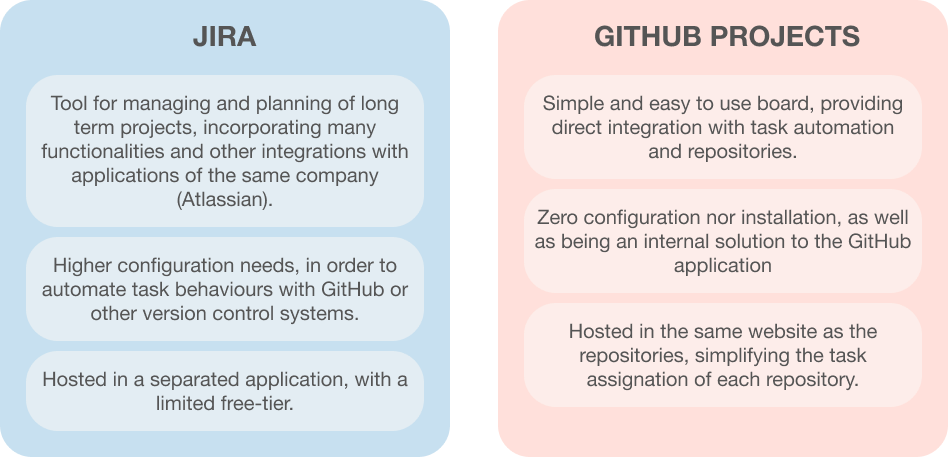
\includegraphics[width=0.85\textwidth]{./assets/jira-vs-github.png}
	\caption{Comparison between Jira and GitHub projects}
\end{figure}
The features of Jira simplified in the above chart, present it as a
task-managing tool for more complex projects. However, considering the specific
development characteristics of this project, it is clear that the time
constraints play an important role in preferring one tool over the other. This
is a short-term project, and requires a mangement tool that primarly allows the
organization of issues and provides an easy visualisation. Nonetheless, GitHub
projects can be scalable to bigger projects, which would allow future teams to
keep using it as their task-managing tool.
\\
Therefore, the features provided by GitHub Projects's boards, as an adaptable
and flexible tool that enables tracking and planning of work within the code
repository, are ideal for the execution of this project. It also facilitates the
organization of tasks and provides a straightforward way to visualise the status
of their resolution.
\section{GitHub Projects}
\subsection{Team organization}
In order to properly develop the project, the GitHub organization members have
been divided in two teams. The \emph{backend} team consisting of the
three\footnote{Adrià Manero, Luisa Salazar and Carlos Jefferson} members with
backend related tasks. The \emph{frontend} team consisting of the
member\footnote{Miquel de Domingo} with frontend related tasks.
\begin{figure}[H]
	\centering
	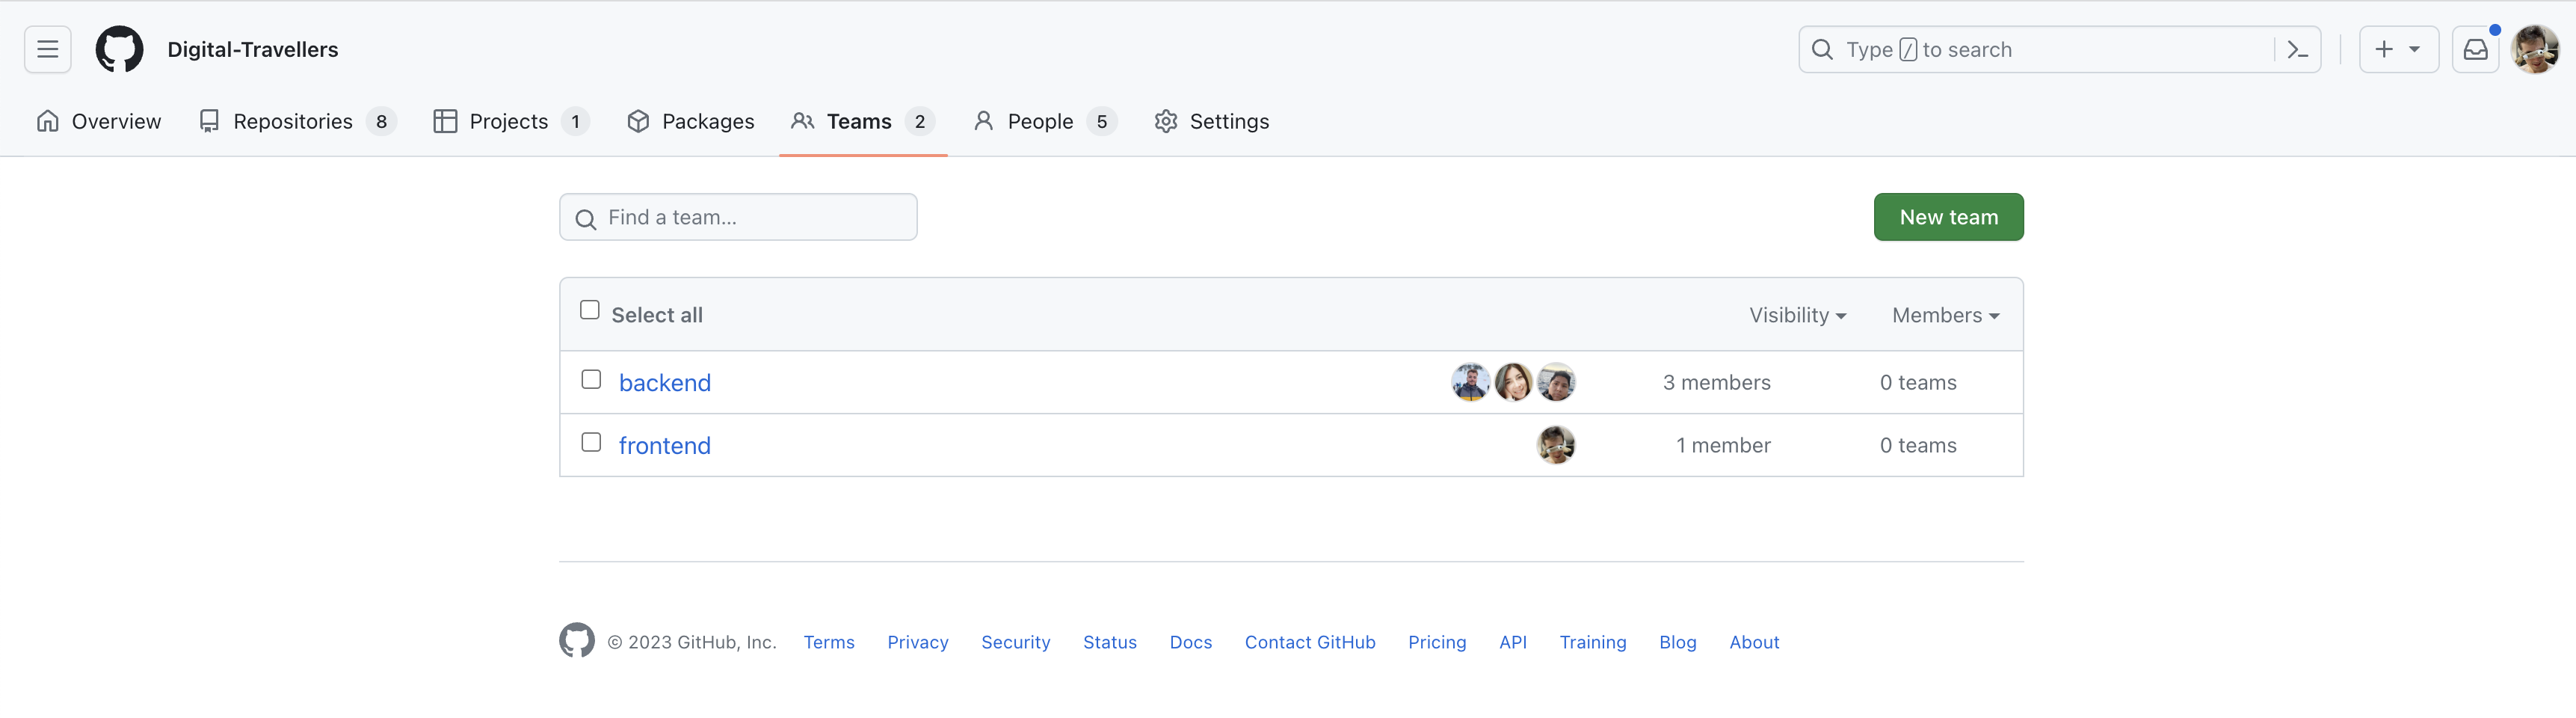
\includegraphics[width=\textwidth]{./assets/gh-teams.png}
	\caption{Comparison between Jira and GitHub projects}
\end{figure}
The goal of having projects within the project is to reflect the structure of
the team with mentions and permissions in a cascade format. The members of each
team can send notifications to an entire team or ask for reviews for a team.
There, each member of the team will receive the notiication. GitHub
organizations allow the creating of teams, which can have sub-teams within. In
the current team structure, such nested level is not required.
\subsection{Board view}
The board of a project is what allows the developers to visualise the state of
the project. It can accept from issues defined in the board (not linked to any
repository), issues linked to a repository and even pull requests, specific for
a repository aswell. It also allows filtering and grouping by many different
options. This filtering and grouping can also be stored as views in a separate
tab.
\begin{figure}[H]
	\centering
	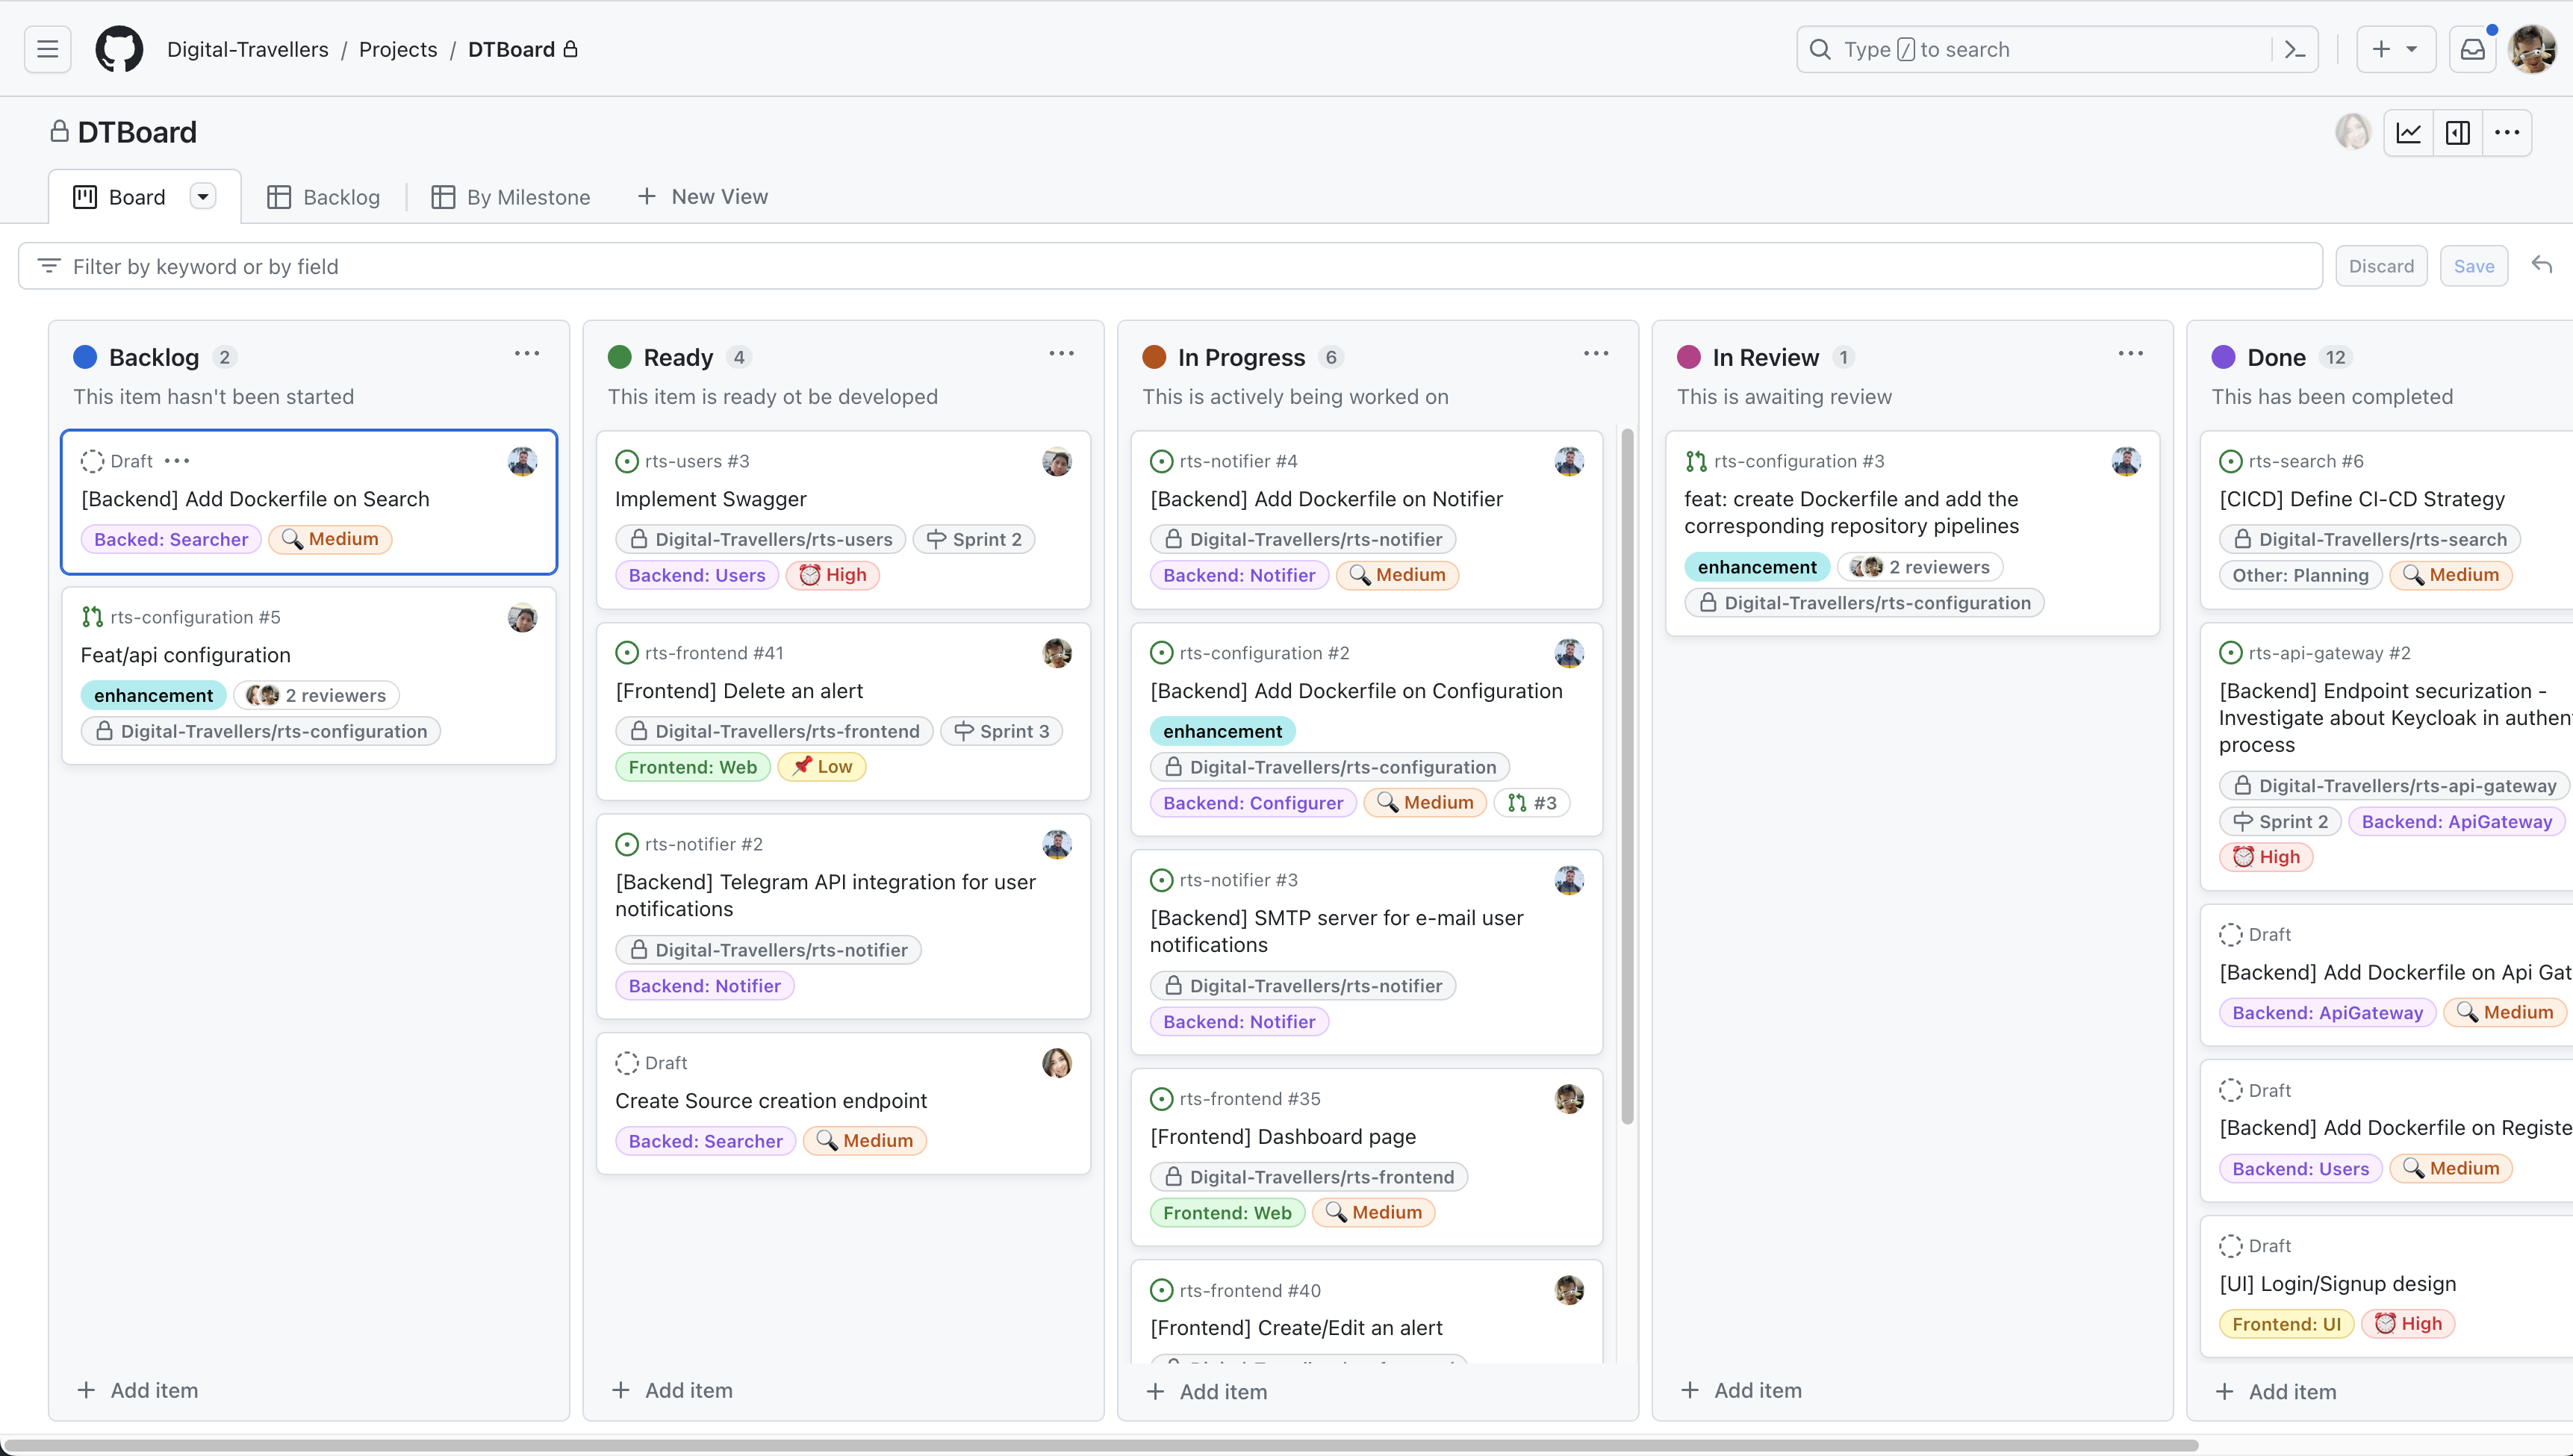
\includegraphics[width=\textwidth]{./assets/gh-board.png}
	\caption{Visualisation of the board}
\end{figure}
Since GitHub does not have the concept of sprints, the team has used milestones
as an alternative to defining the sprints. Even though milestones are repository
specific, they can be grouped for different repositories as long as they have
the same name.
\begin{figure}[H]
	\centering
	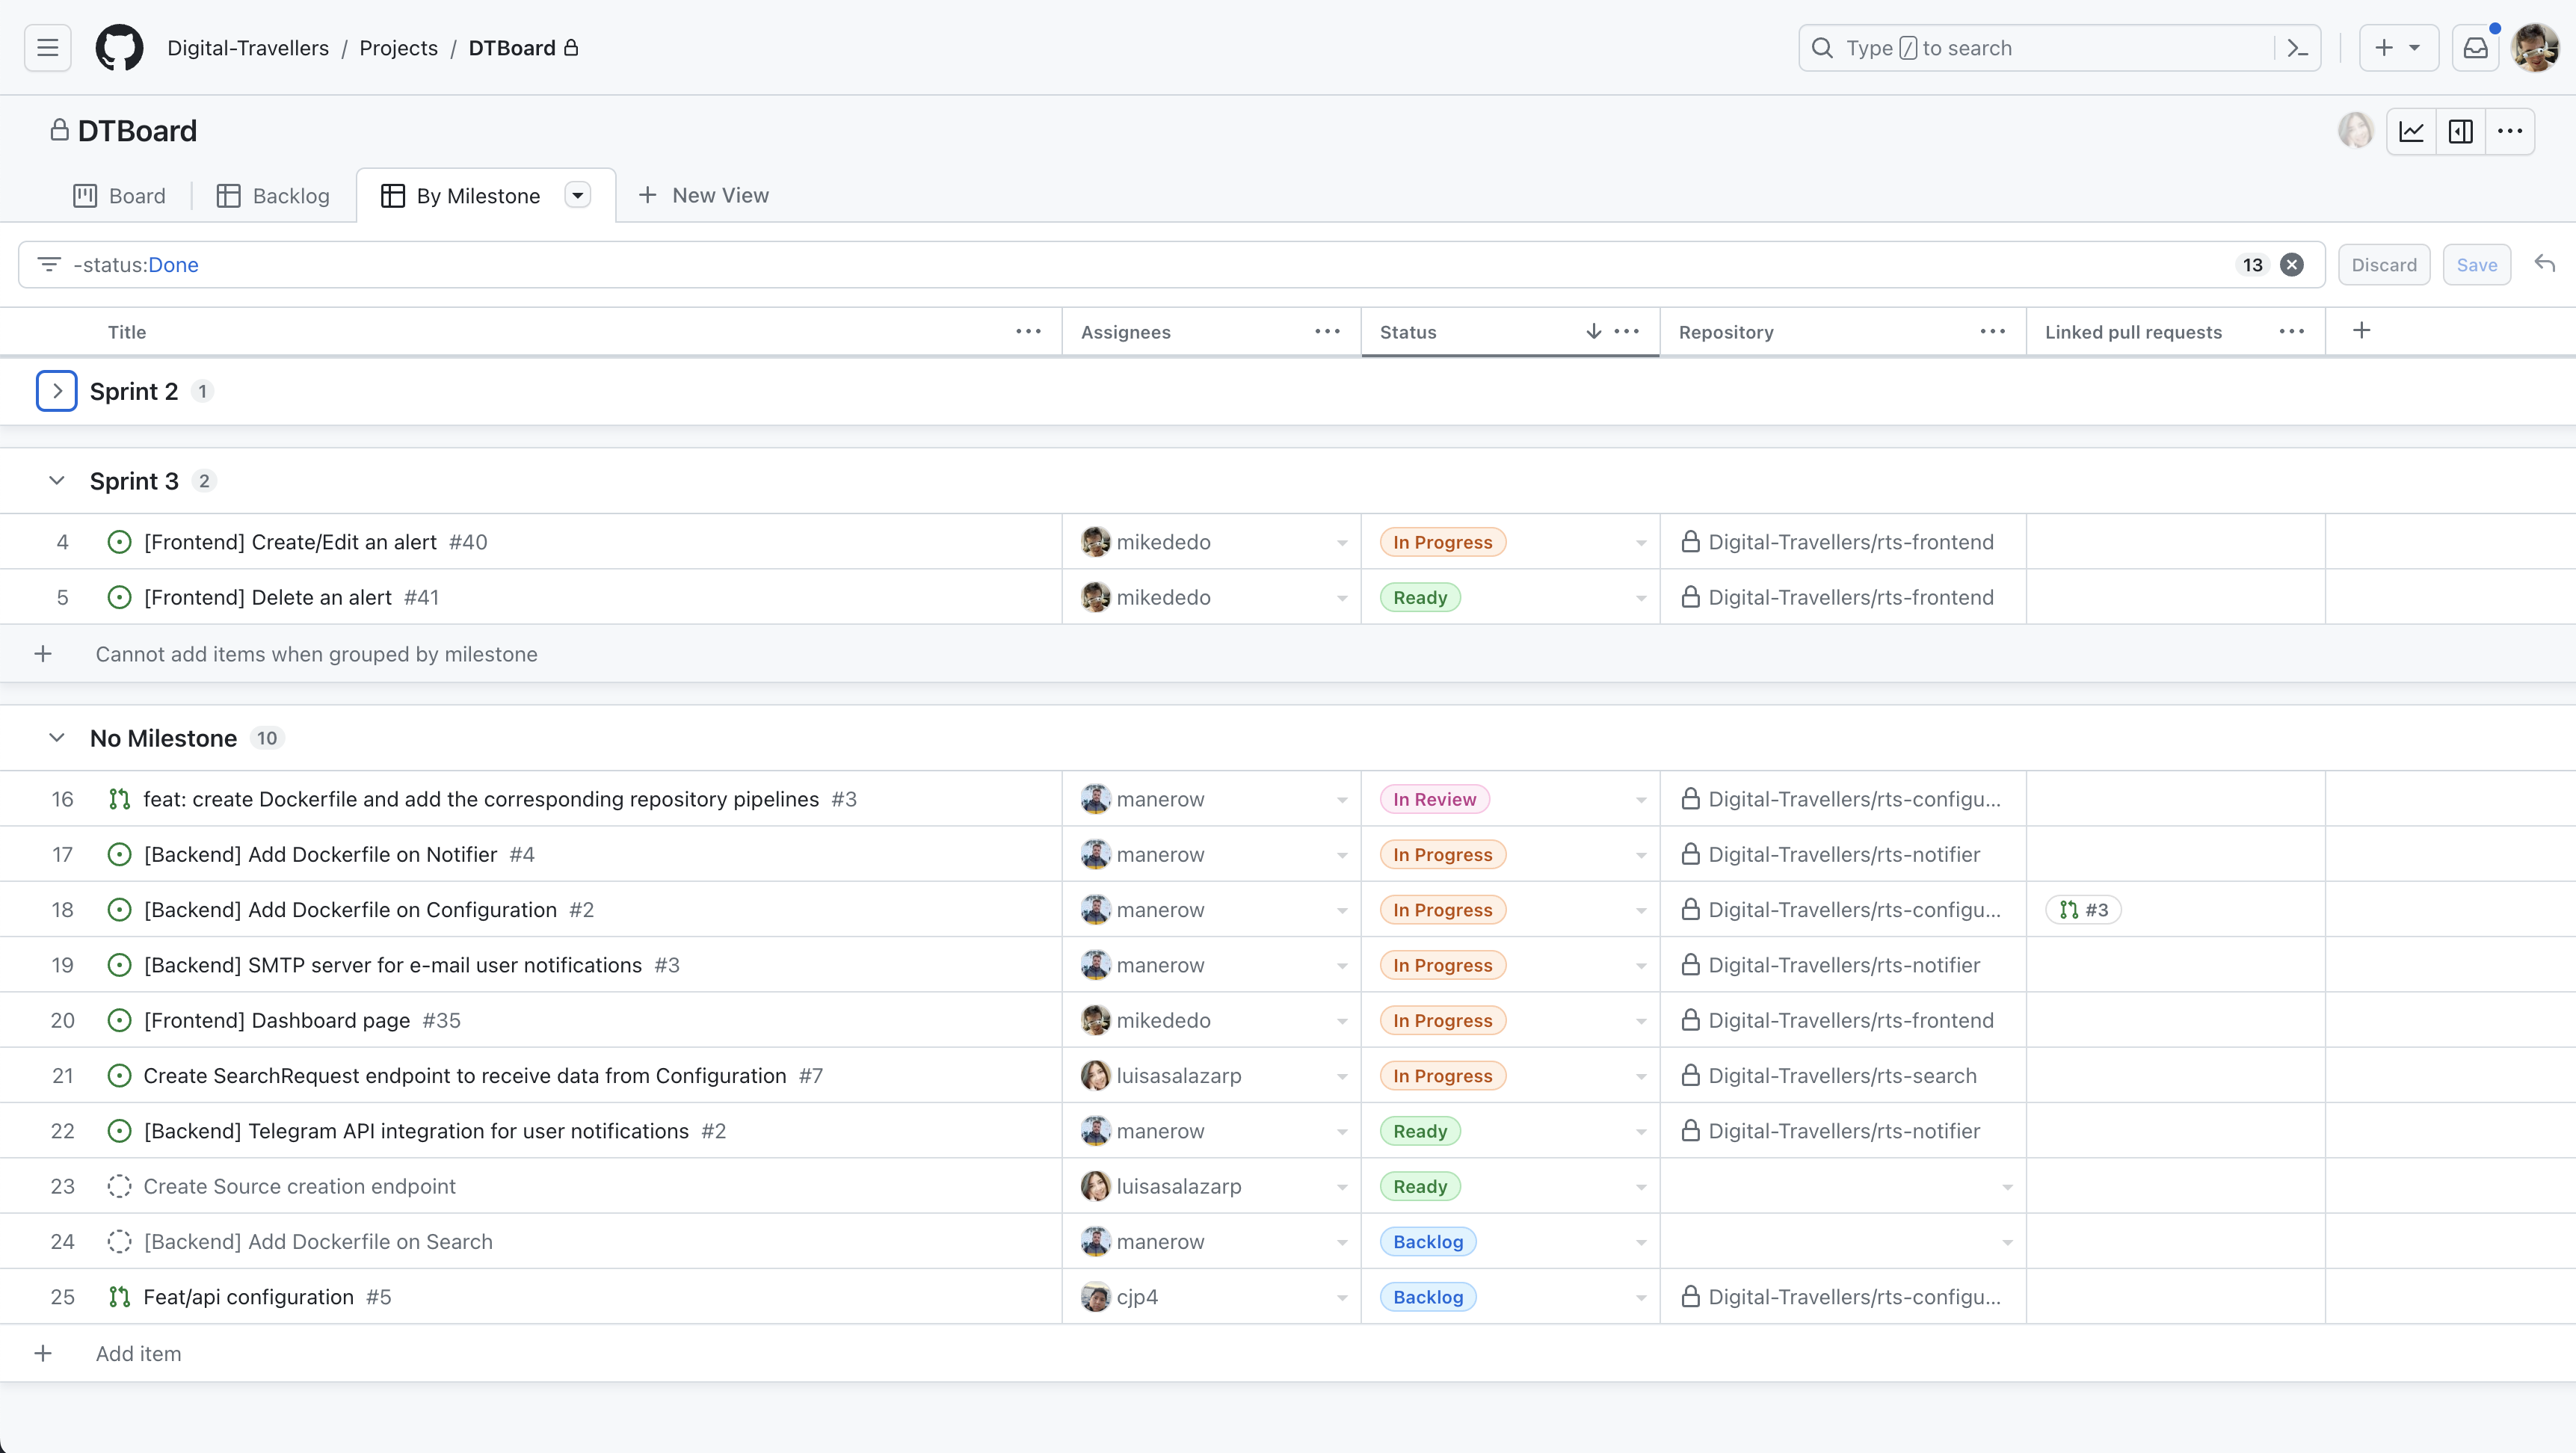
\includegraphics[width=\textwidth]{./assets/gh-board-milestone.png}
	\caption{Visualisation of the board, grouping by milestones}
\end{figure}
Another benefit of directly using the board from GitHub is the possibility of
constantly being up-to-date with the project status, as the project will also be
updated with the activity (creation of pull requests and issues) of each
repository.
\\
It also allows to have personalized field for each ticket, allowing the team to
add extra information just with the visualisation of the ticket. In this case,
the following meta-information has been defined for each ticket:
\begin{enumerate}[label = -]
	\item Status. The status allows the developers to know if the ticket is in the
	      backlog, ready to be developed, in progress, in review or waiting to be
	      reviewed, and done, in case the ticket has been merged successfully.
	\item Project. A small tag that gives information to which project the ticket
	      is related.
	\item Priority. It allows to know which tickets should be prioritised over
	      others.
\end{enumerate}
\end{document}
